% !TEX root = ../om_ts_01.tex

\begin{frame} % frame name
	
	\videotitle{ETS Model (Part I)}
	
\end{frame}



\begin{frame}{ETS Model: Plan}
	\begin{itemize}[<+->]
		\item ETS as a model
		\item Formulas for predictions
		\item Adding a trend
		\item Idea of damped trend
	\end{itemize}
	
\end{frame}




\begin{frame}
	\frametitle{How many ETS models in total?}
	
	ETS — \alert{Error, Trend, Seasonality} (error, trend, seasonality)
	
	\pause
	
	\alert{Error}: A, M
	
	\alert{Trend}: N, A, Ad, M, Md
	
	\alert{Seasonality}: N, A, M
	
	\pause
	A — \alert{additive} component
	
	M — \alert{multiplicative} component
	
	N — no component
	
	d — \alert{damping} for the trend
	
	\pause
	
	Formally: \alert{30 options}
	
\end{frame}


\begin{frame}{Historical names}
	
	ETS(ANN) — simple exponential smoothing
	
	ETS(AAA) —  an additive Holt-Winters method
	
	ETS(AAM) —  the multiplicative Holt-Winters method
	
	ETS(AAdM) — Holt-Winters method with a fading trend
	
\end{frame}




\begin{frame}{ETS(ANN) terminology}
	
	$y_t$ — the observed series;
	
	$\ell_t$ — trend, cleaned series;
	
	$u_t$ — a random error
	
	\pause
	\[
	y_t = \ell_{t-1} + u_t;
	\]
	\pause
	\[
	\ell_t = \ell_{t-1} + \alpha u_t, \text{ starts at } \ell_0;
	\]
	\pause
	\[
	u_t \sim \dN(0;\sigma^2) \text{ and are independent}
	\]
	\pause
	
	Parameters: $\alpha$, $\sigma^2$, $\ell_0$
\end{frame}




\begin{frame}{Recognized?}
	
	ETS(ANN) is a generalization of \alert{random walk}
	\pause
	
	\[
	\begin{cases}
		y_t = \ell_{t-1} + u_t; \\
		\ell_t = \ell_{t-1} + \alpha u_t, \text{ starts at } \ell_0; \\
		u_t \sim \dN(0;\sigma^2) \text{ and are independent} \\
	\end{cases}
	\]
	
	\pause
	Substitute $\alpha = 1$:
	\[
	y_t = \ell_t = \ell_{t-1} + u_t
	\]
	
\end{frame}


\begin{frame}
	\frametitle{Estimation}
	
	\alert{Maximum likelihood method} is used for estimation
	
	\pause
	Main idea: \alert{decompose} the likelihood into a sum
	
	\begin{multline*}
		\ln L(y \mid \theta) = \ln L(y_1 \mid \theta) + \ln L(y_2 \mid y_1, \theta) + \ldots + \\
		+ \ln L(y_T \mid y_{T-1}, \ldots, y_1, \theta),
	\end{multline*}
	
	where $\theta = (\alpha, \ell_0, \sigma^2)$
	
	\pause
	Unfortunately, there are no explicit formulas for the estimators
	
\end{frame}

\begin{frame}
	\frametitle{Forecasting}
	
	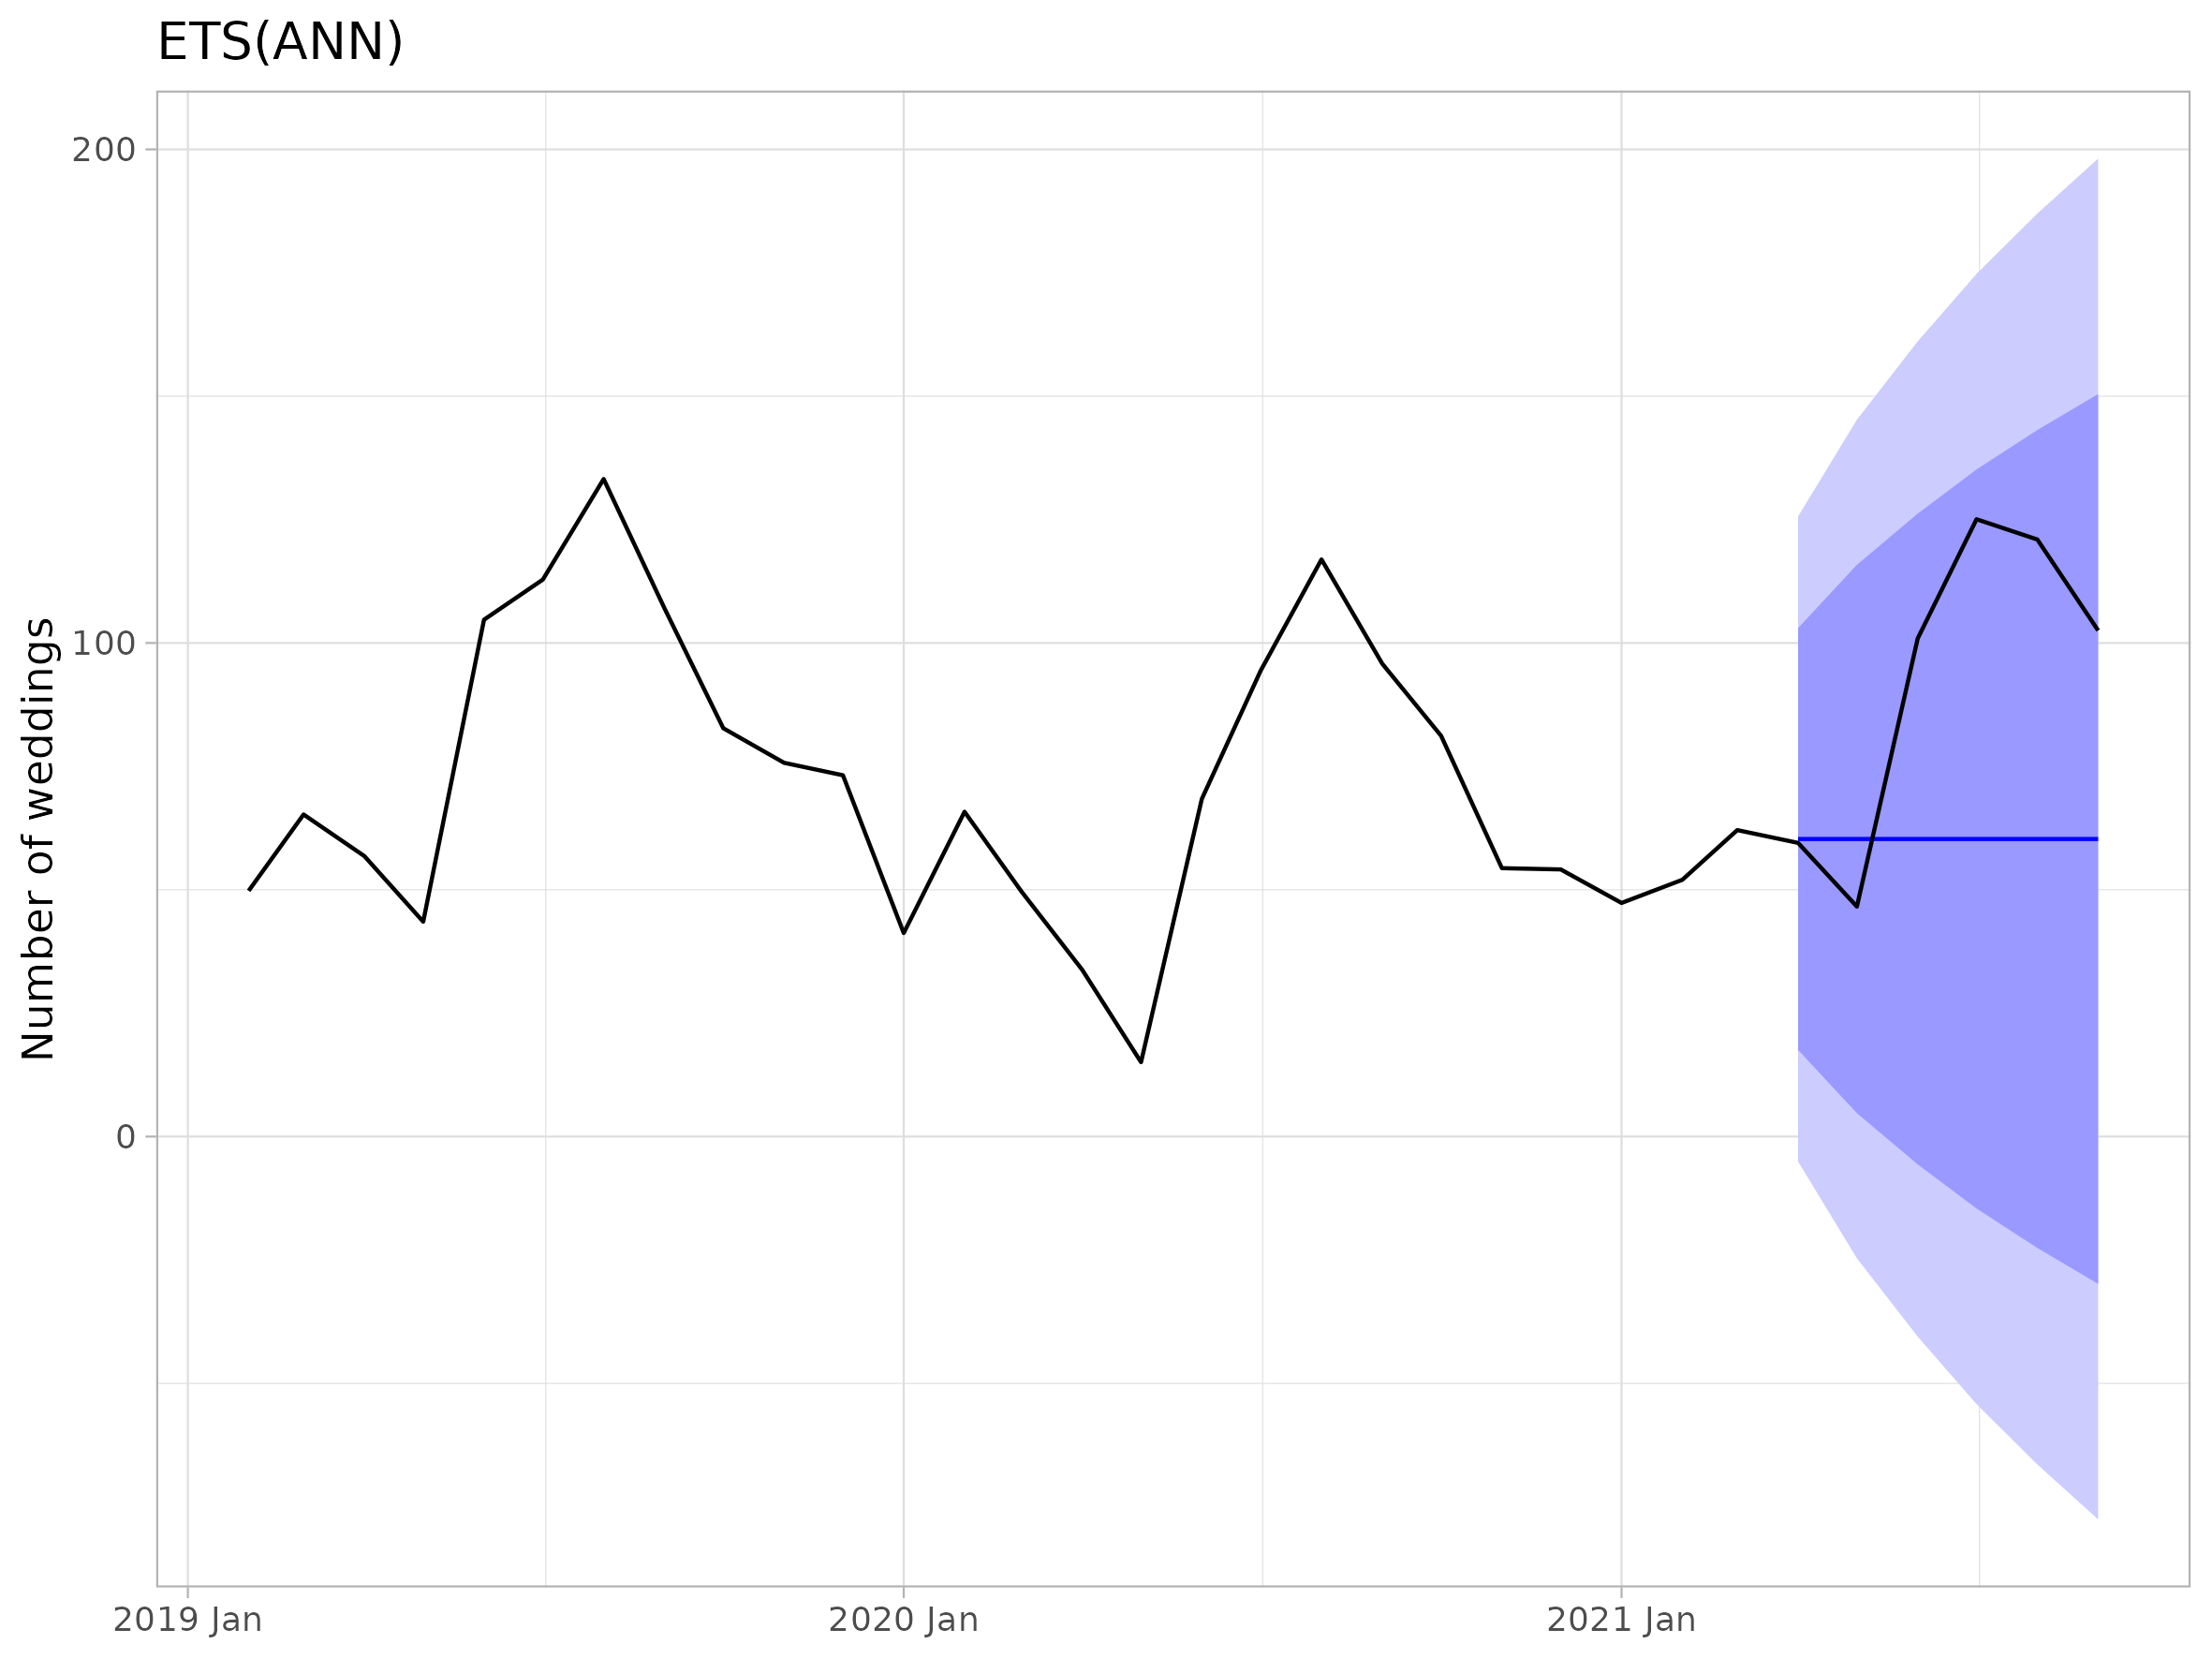
\includegraphics[width=\textwidth]{pictures/om_ts_02-025.png}
	
	
\end{frame}


\begin{frame}
	\frametitle{Forecast 1 step ahead}
	
	Luckily, there are \alert{recurrent formulas} for predictions
	\pause
	
	\[
	\begin{cases}
		y_t = \ell_{t-1} + u_t; \\
		\ell_t = \ell_{t-1} + \alpha u_t, \text{ starts at } \ell_0; \\
		u_t \sim \dN(0;\sigma^2) \text{ and are independent}\\
	\end{cases}
	\]
	\pause
	\[
	y_{T+1} = \ell_T + u_{T+1}
	\]
	\pause
	\[
	(y_{T+1} \mid \mathcal F_T) \sim \dN(\ell_T; \sigma^2)
	\]
	
\end{frame}


\begin{frame}
	\frametitle{Forecast 2 steps ahead}
	
	\[
	\begin{cases}
		y_t = \ell_{t-1} + u_t;\\
		\ell_t = \ell_{t-1} + \alpha u_t, \text{ starts at } \ell_0; \\
		u_t \sim \dN(0;\sigma^2) \text{ and are independent}\\
	\end{cases}
	\]
	\pause
	\[
	y_{T+2} = \ell_{T+1} + u_{T+2} = \ell_T + \alpha u_{T+1} + u_{T+2}
	\]
	\pause
	\[
	(y_{T+2} \mid \mathcal F_T) \sim \dN(\ell_T; \sigma^2(\alpha^2 + 1))
	\]
	
\end{frame}

\begin{frame}{Predictive intervals}
	
	From distribution law
	\[
	(y_{T+2} \mid \mathcal F_T) \sim \dN(\ell_T; \sigma^2(\alpha^2 + 1))
	\]
	we can derive a \pause \alert{predictive interval}
	\[
	[\hat\ell_T - 1.96 \hat\sigma \sqrt{\hat\alpha^2 + 1}; \hat \ell_T + 1.96 \hat\sigma \sqrt{\hat\alpha^2 + 1}].
	\]
\end{frame}


\begin{frame}
	\frametitle{What was discovered in the 1950s?}
	
	\[
	\begin{cases}
		y_t = \ell_{t-1} + u_t;\\
		\ell_t = \ell_{t-1} + \alpha u_t, \text{ starts at } \ell_0 \\
	\end{cases}
	\]
	\pause
	Let's rewrite the second equation:
	\[
	\ell_t = \ell_{t-1} + \alpha (y_t - \ell_{t-1}) = \alpha y_t + (1 - \alpha) \ell_{t-1}
	\]
	
	\pause
	\alert{Simple exponential smoothing}:
	
	\[
	\hat\ell_1 = y_1
	\]
	\pause
	\[
	\hat \ell_t = \alpha y_t + (1-\alpha) \hat \ell_{t-1}
	\]
	\pause
	\[
	\min_{\alpha} \sum (y_t - \hat \ell_t)^2
	\]
	
\end{frame}







\begin{frame}
	\frametitle{Adding trend!}
	
	$y_t$ — the observed series;
	
	$\ell_t$ — trend, cleaned series;
	
	$b_t$ — current growth rate of the cleaned series;
	
	$u_t$ — a random error
	
	\pause
	ETS(AAN):
	
	A — \alert{additive} error;
	
	A — \alert{additive} trend;
	
	N — \alert{no} seasonality
	
\end{frame}

\begin{frame}
	\frametitle{ETS(AAN): equations}
	
	
	\[
	\begin{cases}
		y_t = \ell_{t-1} + \alert{b_{t-1}} + u_t; \\
		\ell_t = \ell_{t-1} + \alert{b_{t-1}} + \alpha u_t, \text{ starts at } \ell_0; \\
		u_t \sim \dN(0;\sigma^2) \text{ and are independent} \\
		\alert{b_t = b_{t-1} + \beta u_t},\text{ starts at } b_0; \\
	\end{cases}
	\]
	
	
	Parameters: $\alpha$, $\beta$, $\sigma^2$, $\ell_0$, $b_0$
	
	
\end{frame}

\begin{frame}
	\frametitle{ETS(AAN): Forecasting}
	
	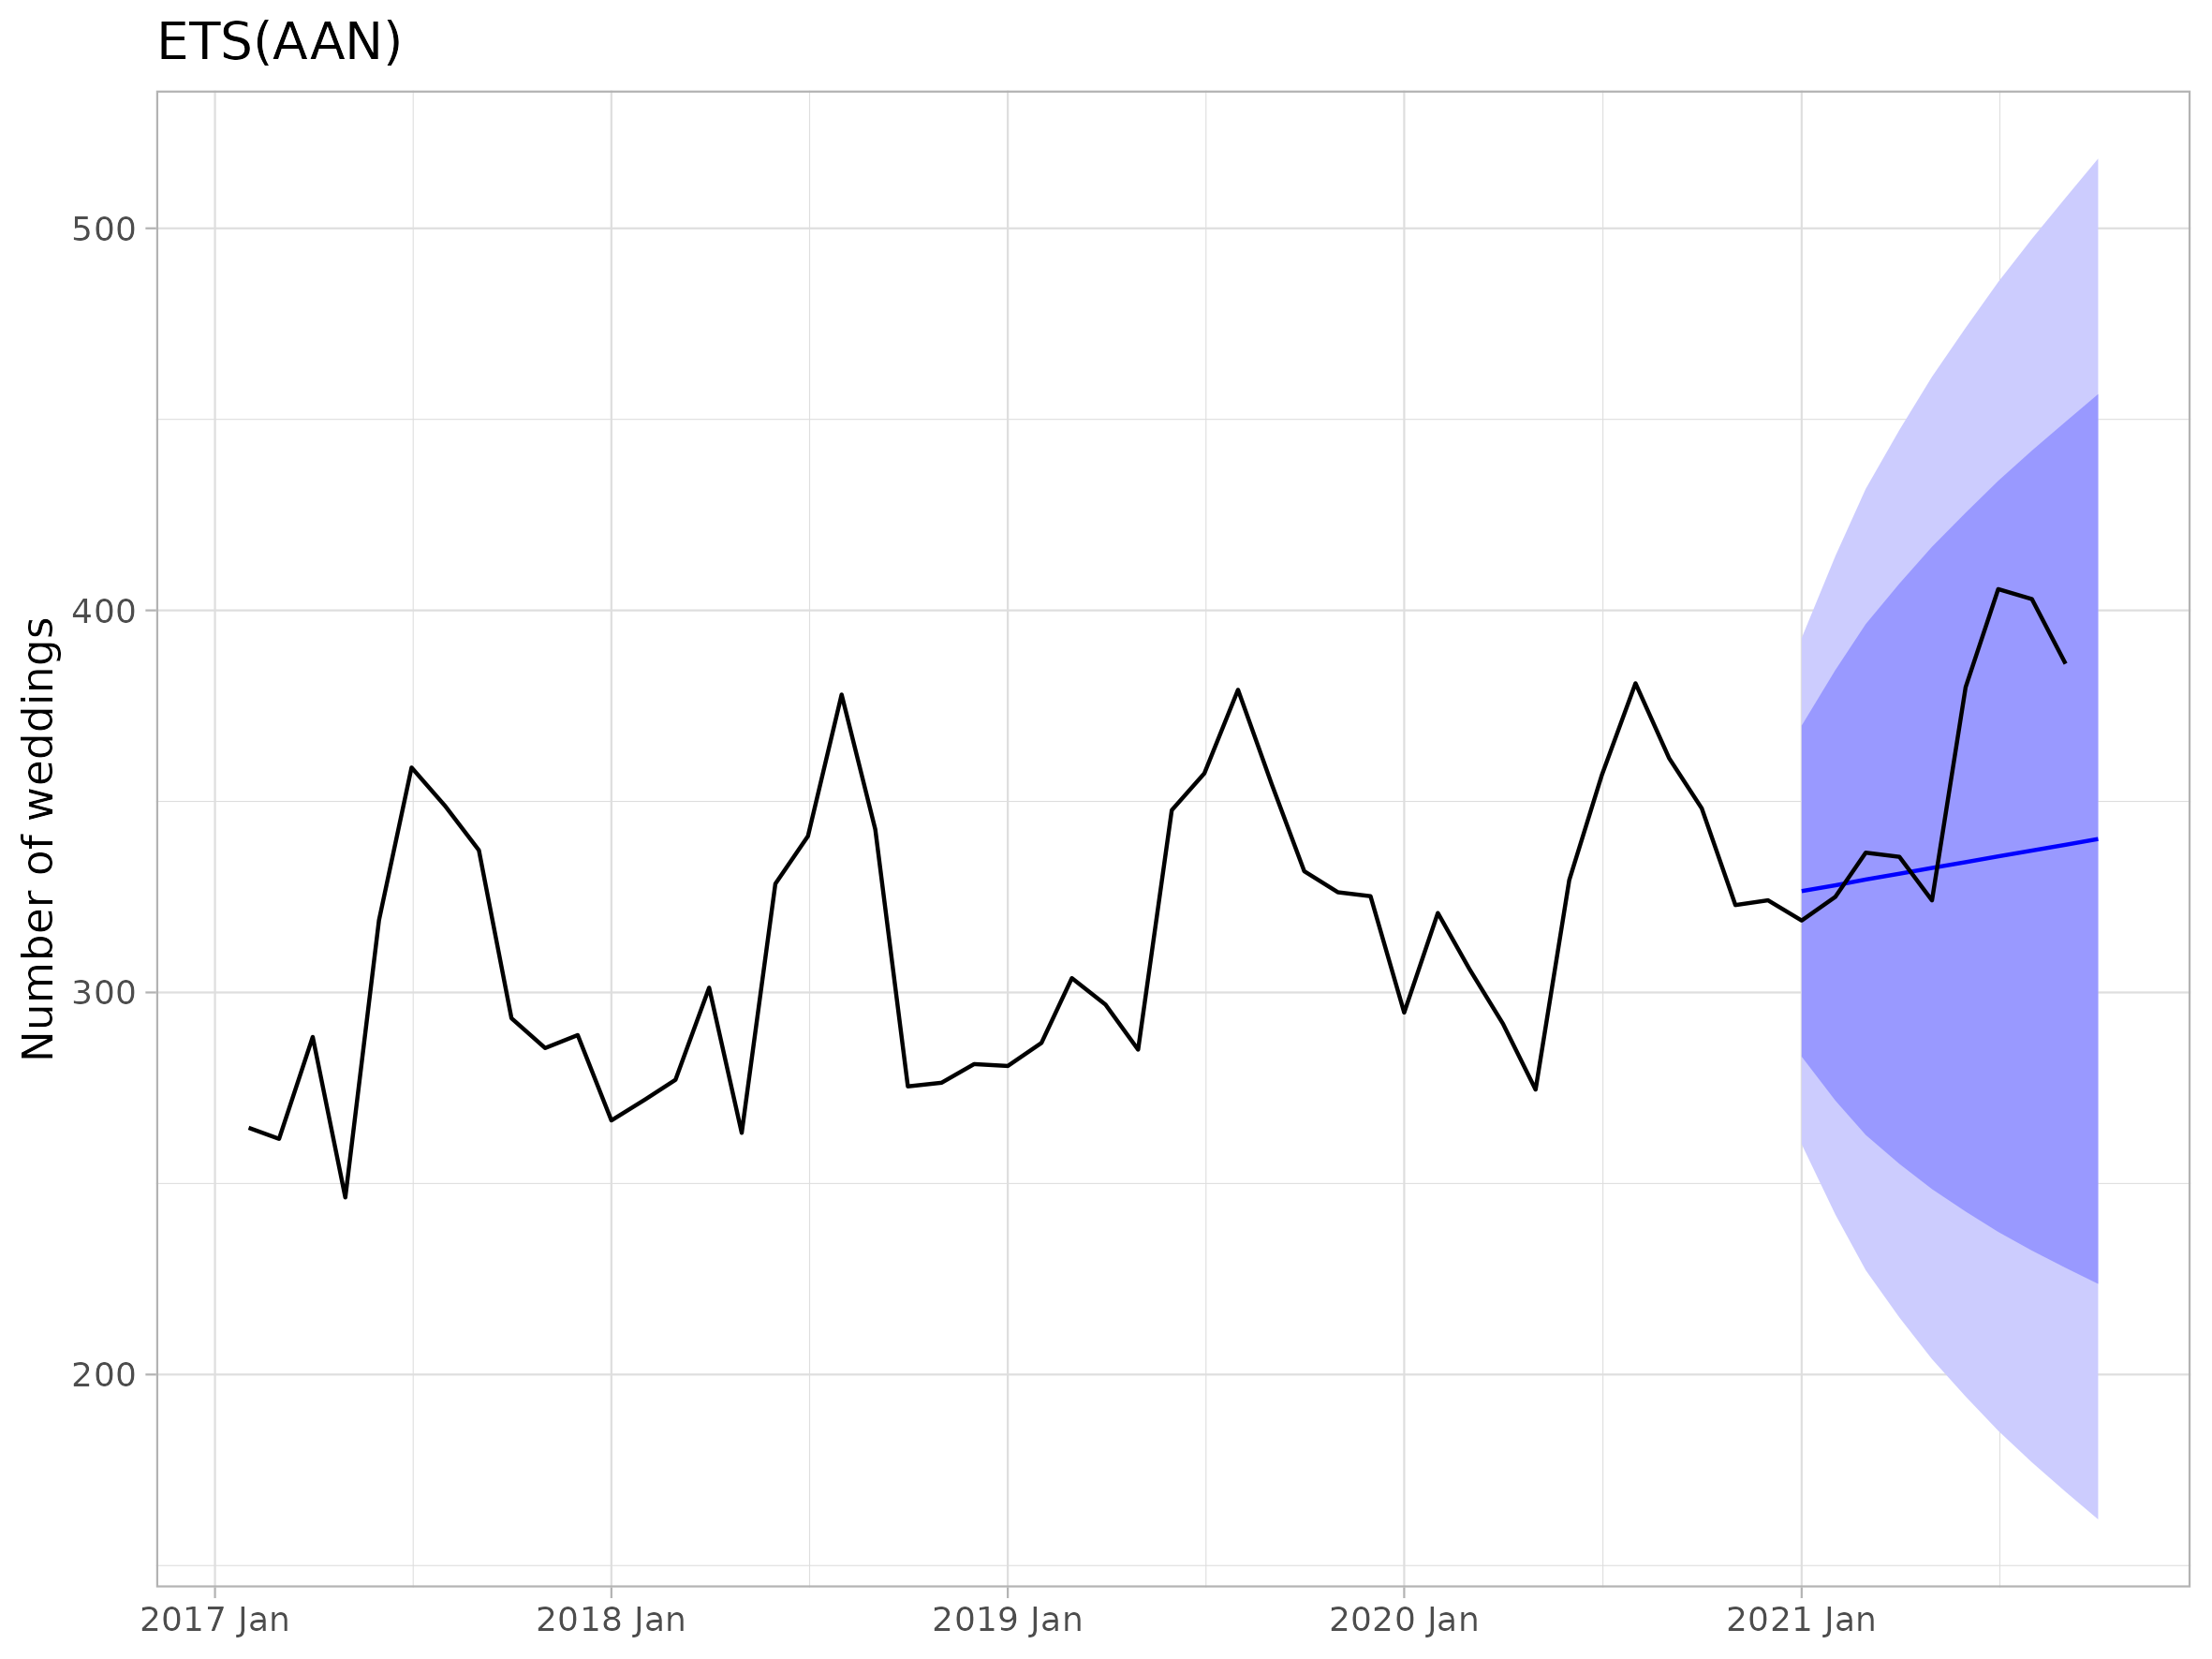
\includegraphics[width=\textwidth]{pictures/om_ts_02-052.png}
	
\end{frame}


\begin{frame}
	\frametitle{Forecast 1 step ahead}
	
	\[
	\begin{cases}
		y_t = \ell_{t-1} + b_{t-1} + u_t; \\
		\ell_t = \ell_{t-1} + b_{t-1} + \alpha u_t, \text{ starts at } \ell_0; \\
		u_t \sim \dN(0;\sigma^2) \text{ and are independent.} \\
		b_t = b_{t-1} + \beta u_t,\text{ starts at } b_0 \\
	\end{cases}
	\]
	
	\[
	y_{T+1} = \ell_T + b_T + u_{T+1}
	\]
	
	\[
	(y_{T+1} \mid \mathcal F_T) \sim \dN(\ell_T + b_T; \sigma^2)
	\]
	
\end{frame}


\begin{frame}
	\frametitle{Forecast 2 steps ahead}
	
	\[
	\begin{cases}
		y_t = \ell_{t-1} + b_{t-1} + u_t; \\
		\ell_t = \ell_{t-1} + b_{t-1} + \alpha u_t, \text{ starts at } \ell_0; \\
		u_t \sim \dN(0;\sigma^2) \text{ and are independent} \\
		b_t = b_{t-1} + \beta u_t,\text{ starts at } b_0 \\
	\end{cases}
	\]
	
	\begin{multline*}
		y_{T+2} = \ell_{T+1} + b_{T+1} + u_{T+2} = (\ell_T + b_T + \alpha u_{T+1}) +\\
		+ (b_T + \beta u_{T+1}) + u_{T+2}
	\end{multline*}
	
	\[
	(y_{T+2} \mid \mathcal F_T) \sim \dN(\ell_T + 2b_T; \sigma^2((\alpha + \beta)^2 + 1))
	\]
	
\end{frame}



\begin{frame}{Problem with trend in ETS(AAN)}
	
	In the ETS(AAN) model \alert{growth rate} of the $\ell_t$ trend is defined by the formula
	\[
	b_t = b_{t-1} + \beta u_t, \text{ starts at } b_0
	\]
	\pause
	Consequently,
	\[
	\E(b_t) = \E(b_{t-1}), \quad \E(b_{T+h} \mid b_T) = b_T
	\]
	\pause
	Long-term forecast of a positive indicator at $b_T < 0$
	will become negative
\end{frame}

\begin{frame}{Contradiction}
	In short-term we expect a change in the indicator:
	
	we \alert{ want a trend} in the model.
	
	\pause
	In long-term negative values are impossible:
	
	we  \alert{don't want a trend} in the model.
	
	\pause
	Solution: \alert{damped} or \alert{fading} trend.
\end{frame}

\begin{frame}{Extra parameters are expensive!}
	We want richer trend dynamics — we need \alert{additional} parameters.
	
	\pause
	Additional parameters — risk \alert{overfitting} of the model,
	\alert{wider confidence intervals} for the remaining parameters.
	
	\pause
	Let's solve the problem  with only \alert{one} new parameter!
\end{frame}

\begin{frame}
	\frametitle{Damped trend}
	
	We introduce the trend damping parameter $\phi \in (0; 1)$ into the slope equation:
	\[
	b_t = \phi b_{t-1} + \beta u_t, \text{ starts at } b_0
	\]
	\pause
	And for the rest of the equations:
	\[
	\begin{cases}
		y_t = \ell_{t-1} + \phi b_{t-1} + u_t; \\
		\ell_t = \ell_{t-1} + \phi b_{t-1} + \alpha u_t, \text{ starts at } \ell_0\\
	\end{cases}
	\]
	
\end{frame}


\begin{frame}{General form of ETS(AAdN)}
	
	\[
	\begin{cases}
		y_t = \ell_{t-1} + \phi b_{t-1} + u_t; \\
		\ell_t = \ell_{t-1} + \phi b_{t-1} + \alpha u_t, \text{ starts at } \ell_0; \\
		b_t = \phi b_{t-1} + \beta u_t, \text{ starts at } b_0; \\
		u_t \sim \dN(0;\sigma^2) \text{ and are independent} \\
	\end{cases}
	\]
	
	
	
	Parameters: $\alpha$, $\sigma^2$, $\ell_0$, $b_0$, $\beta$, $\phi$
\end{frame}

\begin{frame}
	\frametitle{ETS(AAdN): Forecasting}
	
	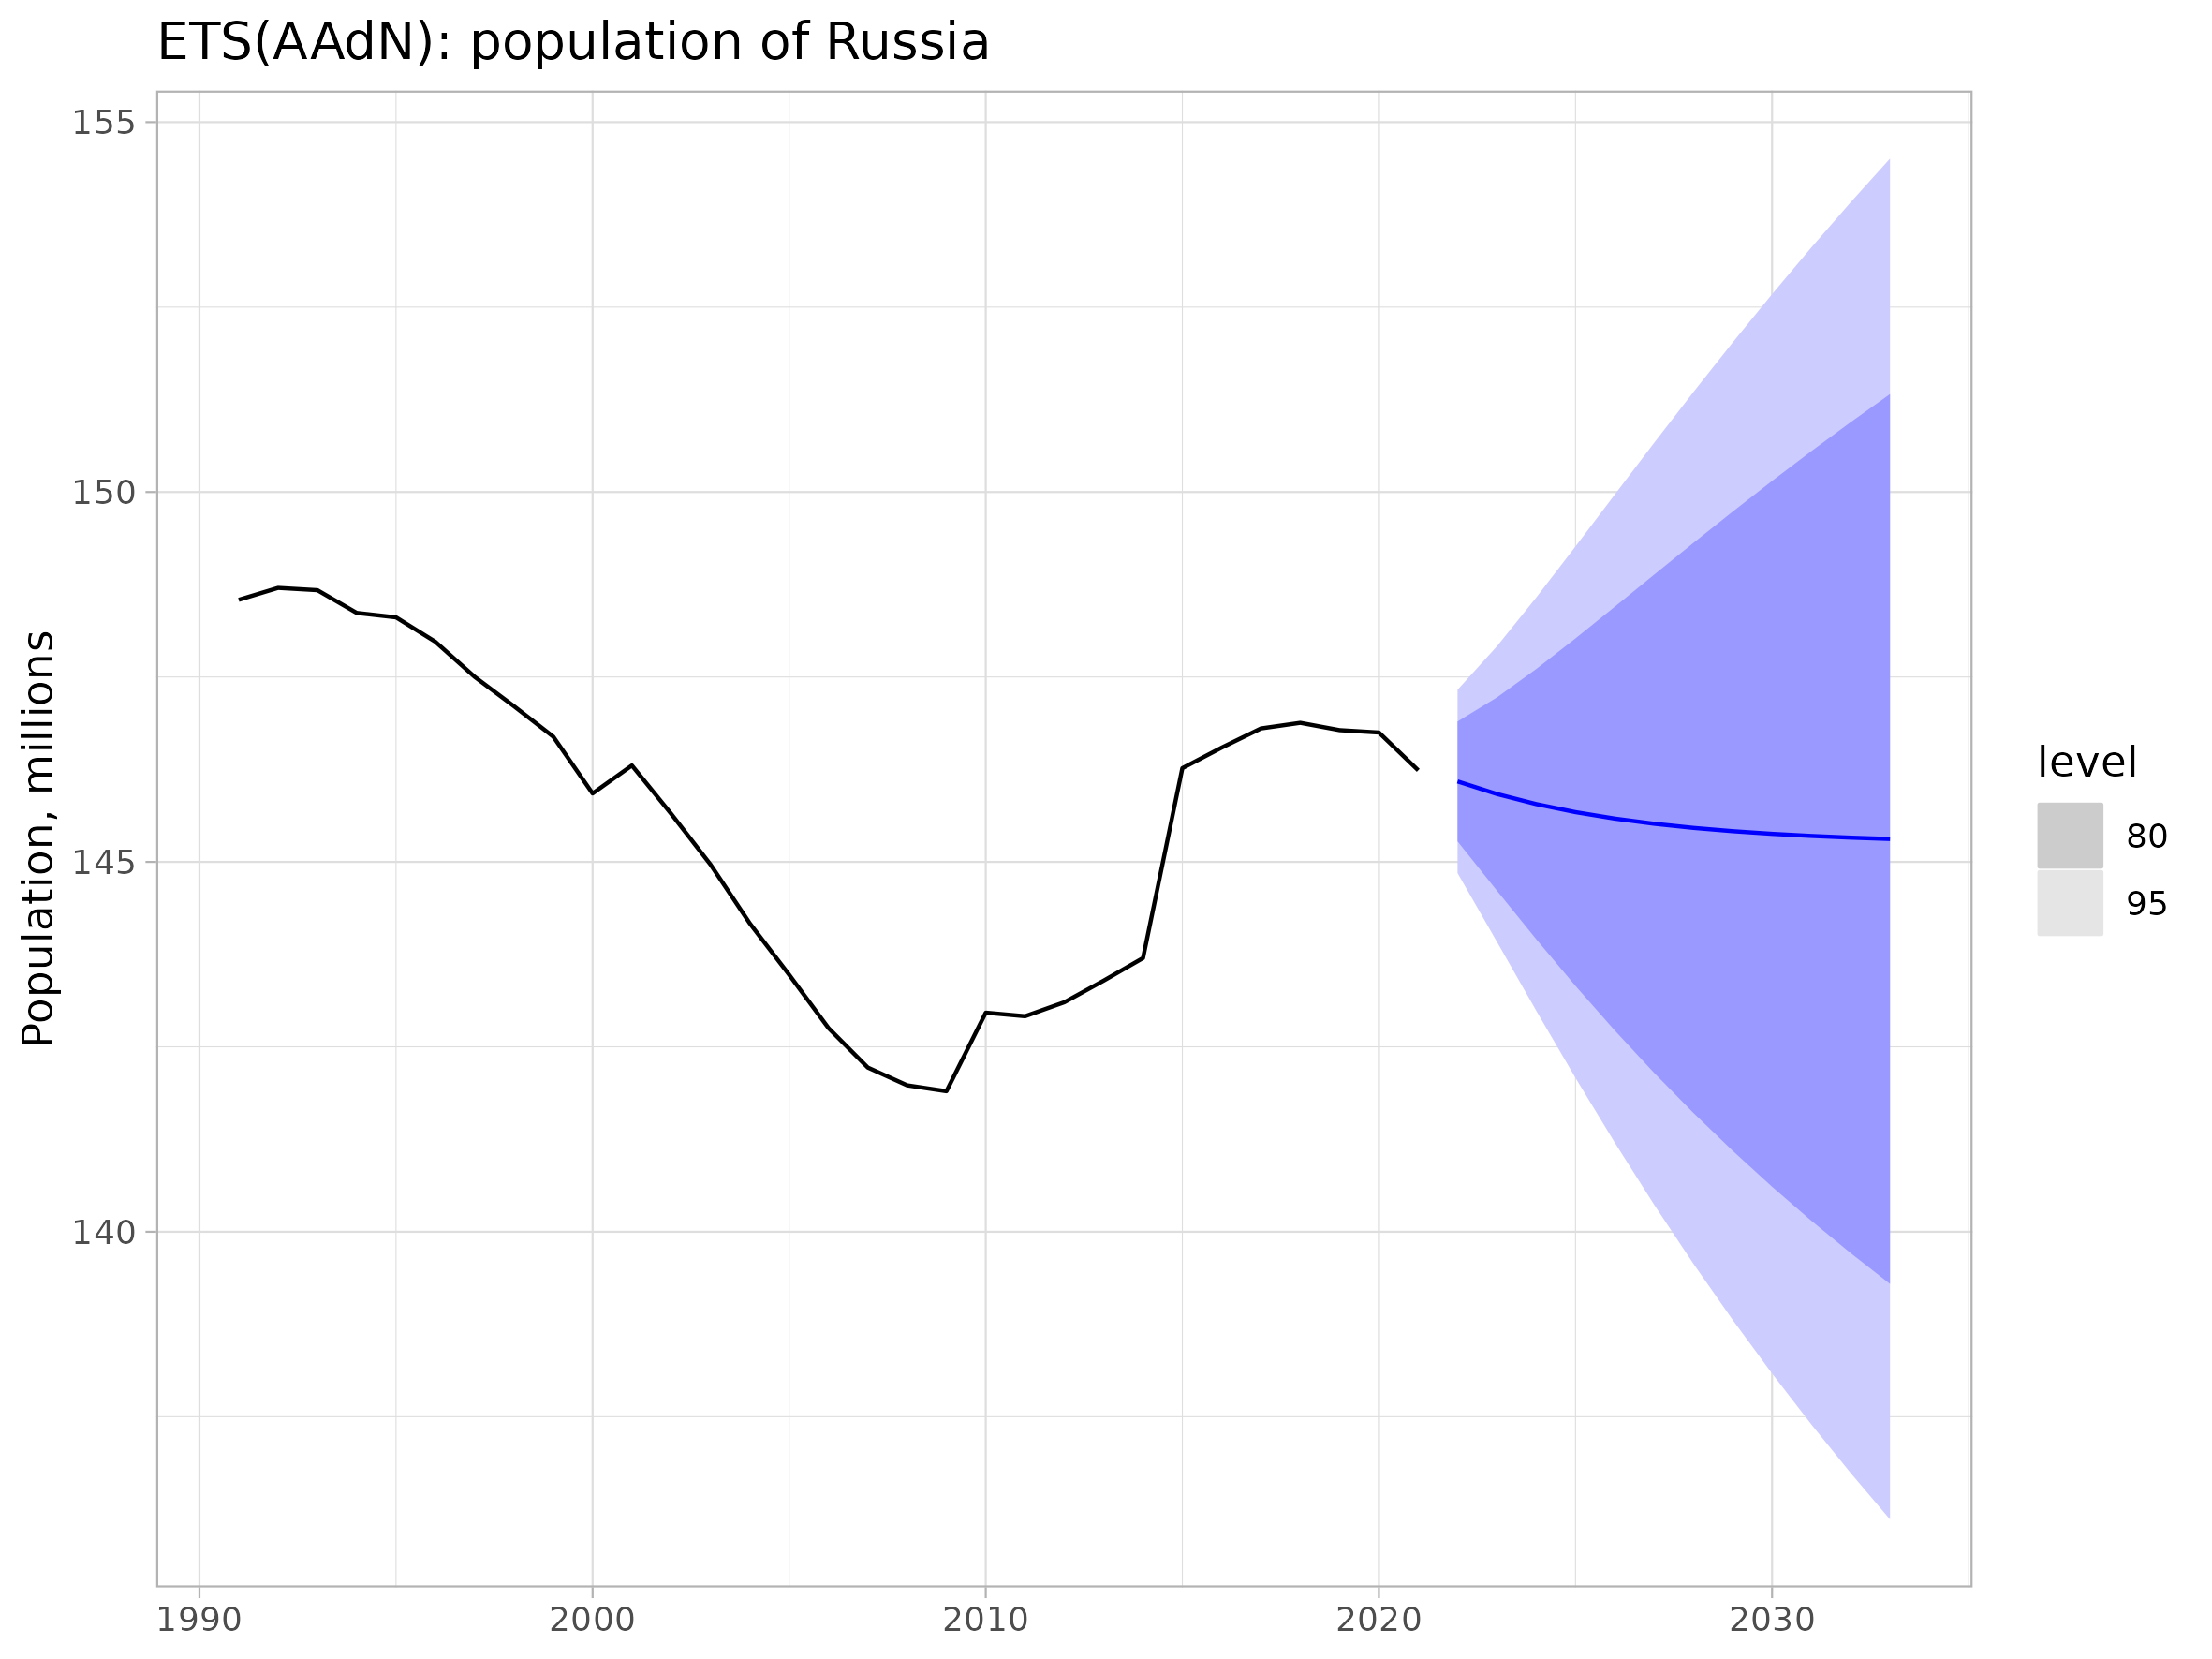
\includegraphics[width=\textwidth]{pictures/om_ts_03-019.png}
	
	% https://www.youtube.com/watch?v=e5WxxvjR9c4
	% I can’t understand what the secret is, if there is a trend, then it doesn’t exist right away.
	
\end{frame}





\begin{frame}{ETS Model: Summary}
	
	\begin{itemize}[<+->]
		\item Formulas for \alert{exponential smoothing} have been around for a long time
		\item ETS — a wide class of modern models
		\item The slope of the trend line can change
		\item Damped trend: on a small forecasting horizon \alert{there is a trend}, on a large horizon — \alert{none}
		
	\end{itemize}
\end{frame}







\begin{frame} % frame name
	
	\videotitle{ETS Model (Part II)}
	
\end{frame}



\begin{frame}{ETS Model: Plan}
	\begin{itemize}[<+->]
		\item Adding seasonality
		\item Formulas for predictions
		\item Decomposition into components
		
		\item Multiplicative components
	\end{itemize}
	
\end{frame}









\begin{frame}
	\frametitle{Adding seasonality!}
	
	$y_t$ — the observed series;
	
	$\ell_t$ — trend, cleaned series;
	
	$b_t$ — current growth rate of the cleaned series;
	
	$s_t$ — seasonal component;
	
	$u_t$ — a random error
	
	\pause
	ETS(AAA):
	
	A — \alert{additive} error;
	
	A — \alert{additive} trend;
	
	A — \alert{additive} seasonality
	
\end{frame}


% TODO: typo with u_t correct on slides!
\begin{frame}
	\frametitle{ETS(AAA): equations}
	
	
	\[
	\begin{cases}
		y_t = \ell_{t-1} + b_{t-1} + \alert{s_{t-12}} + u_t; \\
		\ell_t = \ell_{t-1} + b_{t-1} + \alpha u_t, \text{ starts at } \ell_0; \\
		u_t \sim \dN(0;\sigma^2) \text{ and are independent} \\
		b_t = b_{t-1} + \beta u_t,\text{ starts at } b_0; \\
		\alert{s_t = s_{t-12} + \gamma u_t}; \text{ starts at} s_0, s_{-1}, \ldots, s_{-11}
	\end{cases}
	\]
	
	
	Parameters: $\alpha$, $\beta$, $\gamma$, $\sigma^2$, $\ell_0$, $b_0$, $s_0$, $s_{-1}$, \ldots, $s_ {-11}$
	
	\alert{Restriction}: $s_0 + s_{-1} + \ldots + s_{-11} = 0$
	
	\pause
	
	How many independent parameters are we estimating?
	
	\pause
	
	Correct answer: 17
	
	
\end{frame}



\begin{frame}
	\frametitle{ETS(AAA): Forecasting}
	
	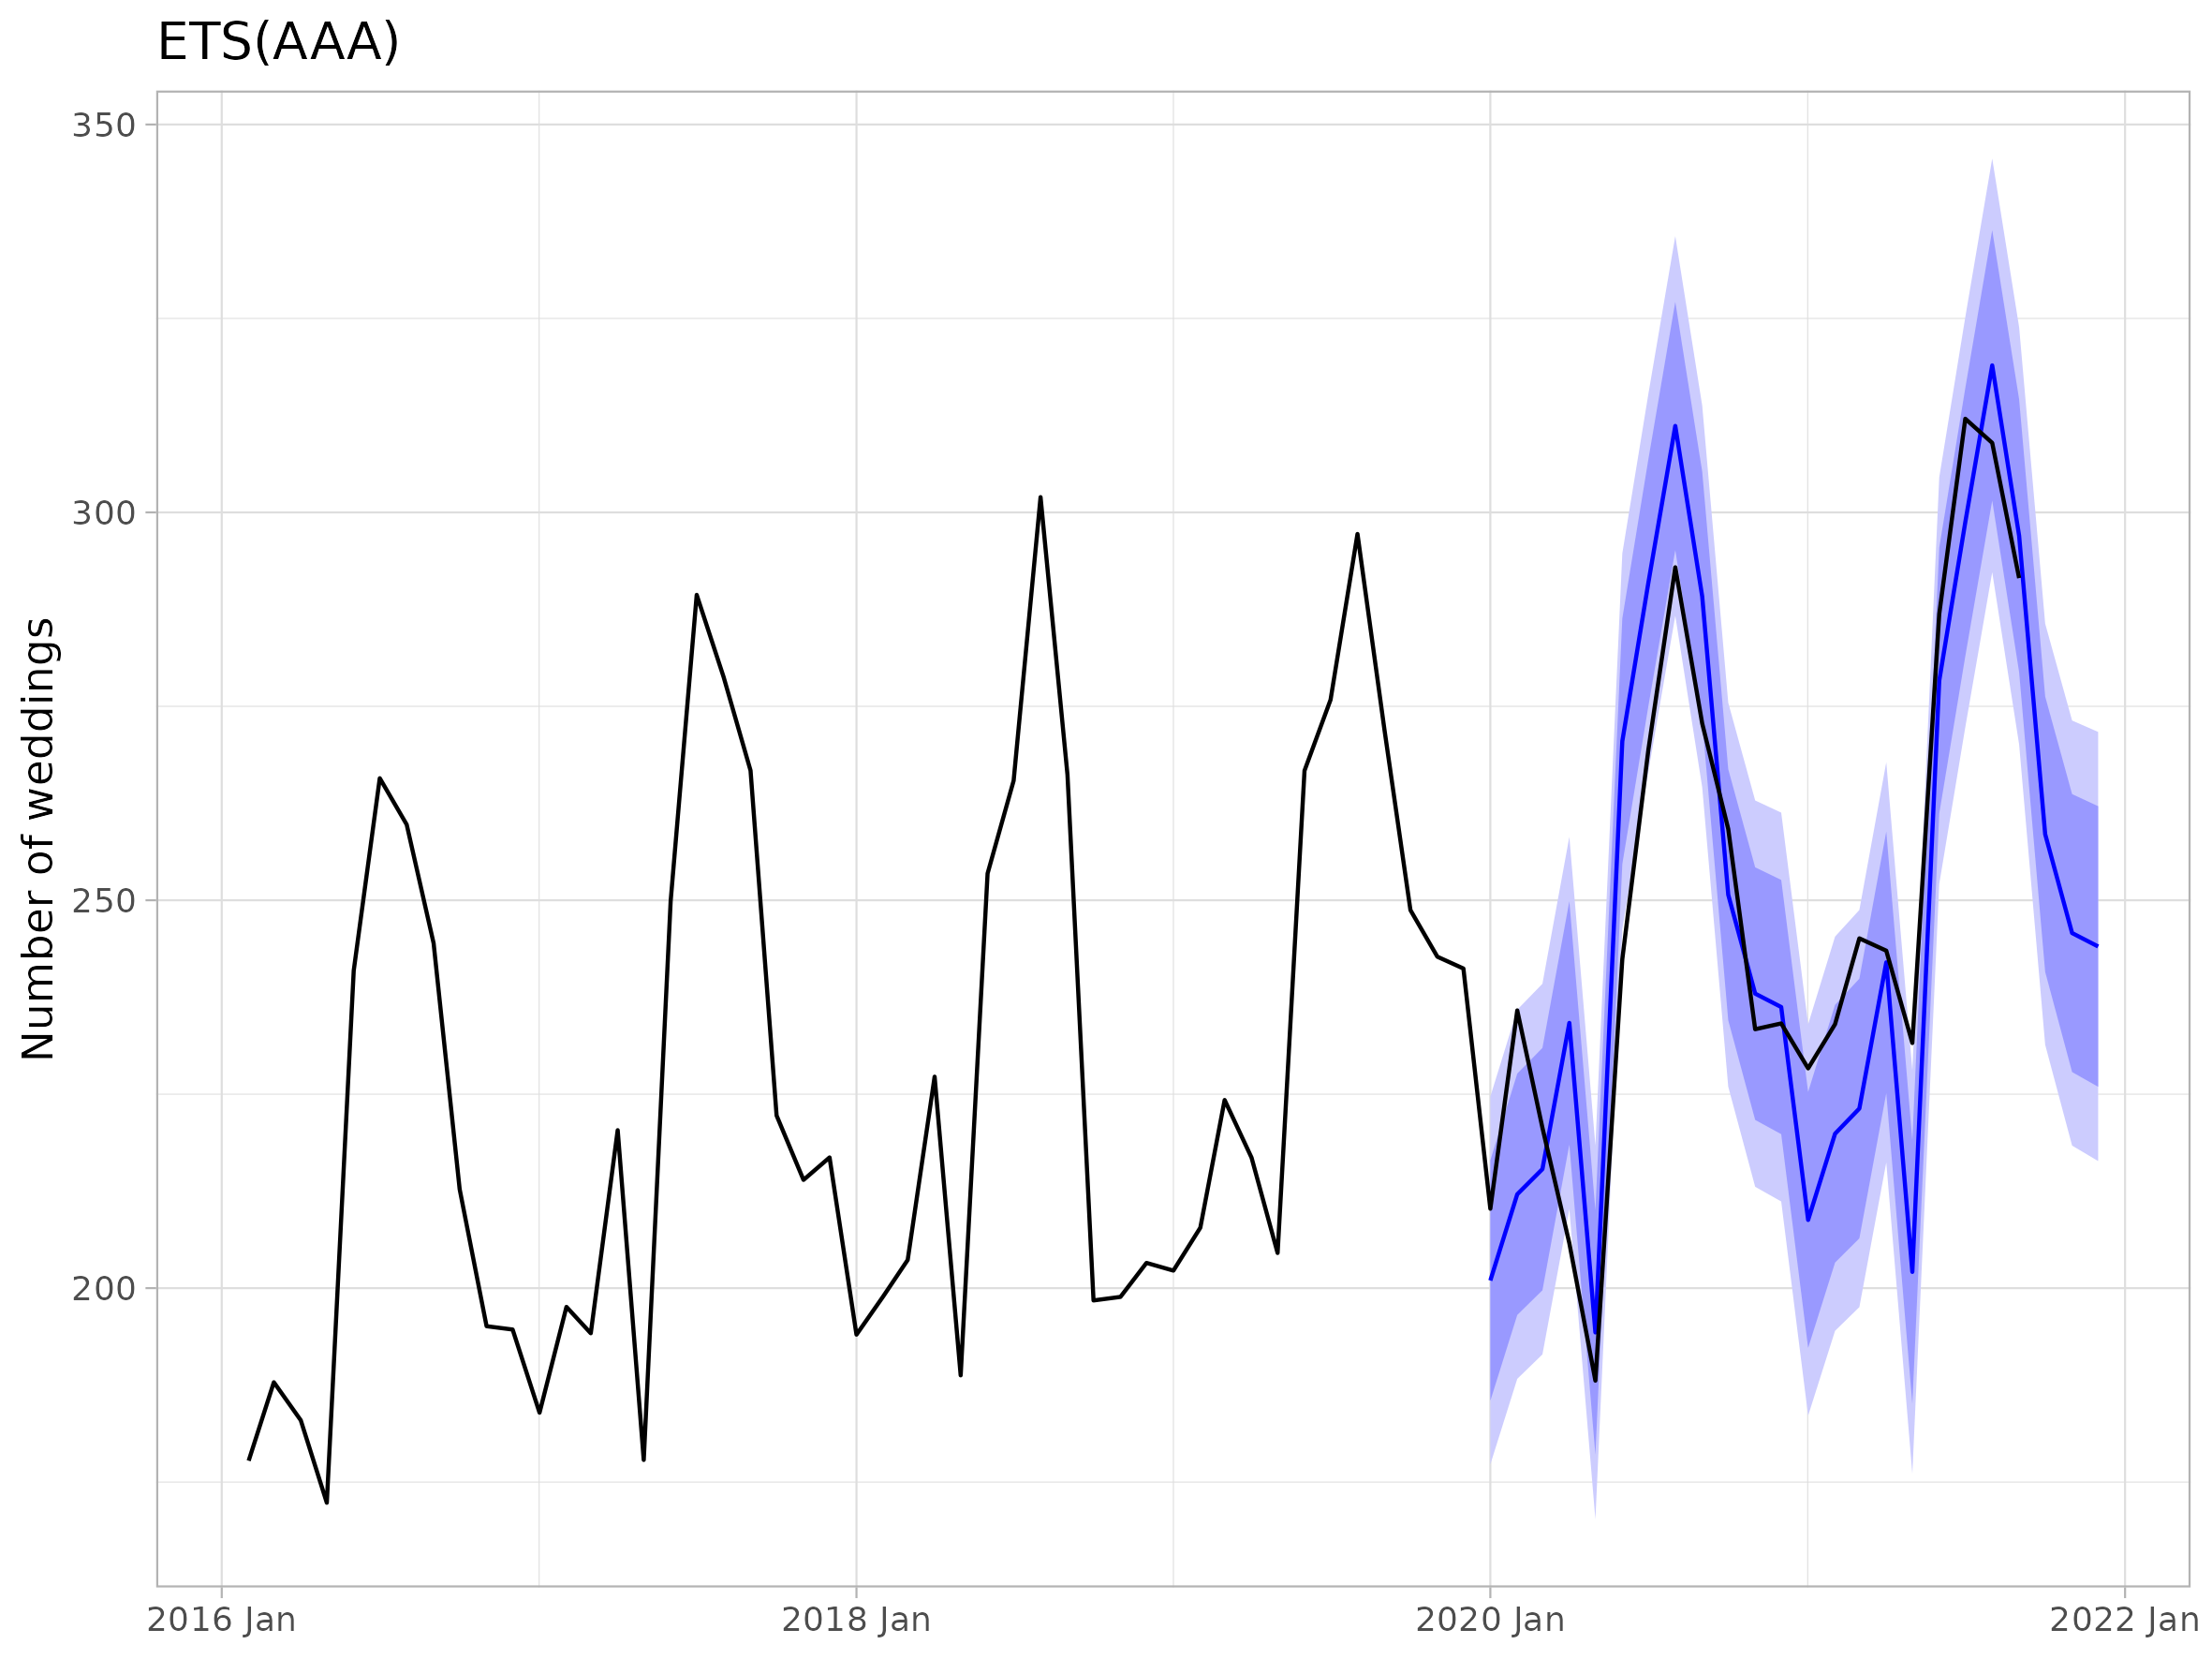
\includegraphics[width=\textwidth]{pictures/om_ts_02-076.png}
	
	
\end{frame}


\begin{frame}
	\frametitle{Forecast 1 step ahead}
	
	\[
	\begin{cases}
		y_t = \ell_{t-1} + b_{t-1} + s_{t-12} + u_t; \\
		\ell_t = \ell_{t-1} + b_{t-1} + \alpha u_t, \text{ starts at } \ell_0; \\
		u_t \sim \dN(0;\sigma^2) \text{ and are independent.} \\
		b_t = b_{t-1} + \beta u_t,\text{ starts at } b_0; \\
		s_t = s_{t-12} + \gamma u_t
	\end{cases}
	\]
	
	\[
	y_{T+1} = \ell_T + b_T + s_{T-11} + u_{T+1}
	\]
	
	\[
	(y_{T+1} \mid \mathcal F_T) \sim \dN(\ell_T + b_T + s_{T-11}; \sigma^2)
	\]
	
\end{frame}


\begin{frame}
	\frametitle{Forecast 2 steps ahead}
	
	\[
	\begin{cases}
		y_t = \ell_{t-1} + b_{t-1} + s_{t-12} + u_t; \\
		\ell_t = \ell_{t-1} + b_{t-1} + \alpha u_t, \text{ starts at } \ell_0; \\
		u_t \sim \dN(0;\sigma^2) \text{ and are independent} \\
		b_t = b_{t-1} + \beta u_t,\text{ starts at } b_0; \\
		s_t = s_{t-12} + \gamma u_t
	\end{cases}
	\]
	
	\begin{multline*}
		y_{T+2} = \ell_{T+1} + b_{T+1} + s_{T-10} + u_{T+2} = (\ell_T + b_T + \alpha u_{T+1} ) +\\
		+ (b_T + \beta u_{T+1}) + s_{T-10} + u_{T+2}
	\end{multline*}
	
	\[
	(y_{T+2} \mid \mathcal F_T) \sim \dN(\ell_T + 2b_T + s_{T-10}; \sigma^2((\alpha + \beta)^2 + 1))
	\]
	
\end{frame}




\begin{frame}
	\frametitle{Decomposition for free!}
	
	Consider the output of ETS(AAA):
	
	\alert{Parameter estimates}: $\hat\alpha$, $\hat\beta$, $\hat\gamma$, $\hat\sigma^2$, $\hat\ell_0$, $\hat b_0$,
	$\hat s_0$, $\hat s_{-1}$, \ldots, $\hat s_{-11}$.
	
	Constraints: $\hat s_0 + \hat s_{-1} + \ldots + \hat s_{-11} = 0$.
	
	\pause
	Estimated \alert{component values}: $\hat \ell_t$, $\hat b_t$, $\hat s_t$.
	
	\pause
	We automatically get \alert{decomposition}: $y_t = \hat \ell_t + \hat s_t + remainder_t$.
	
\end{frame}











\begin{frame}
	\frametitle{Oscillation amplitude can vary}
	
	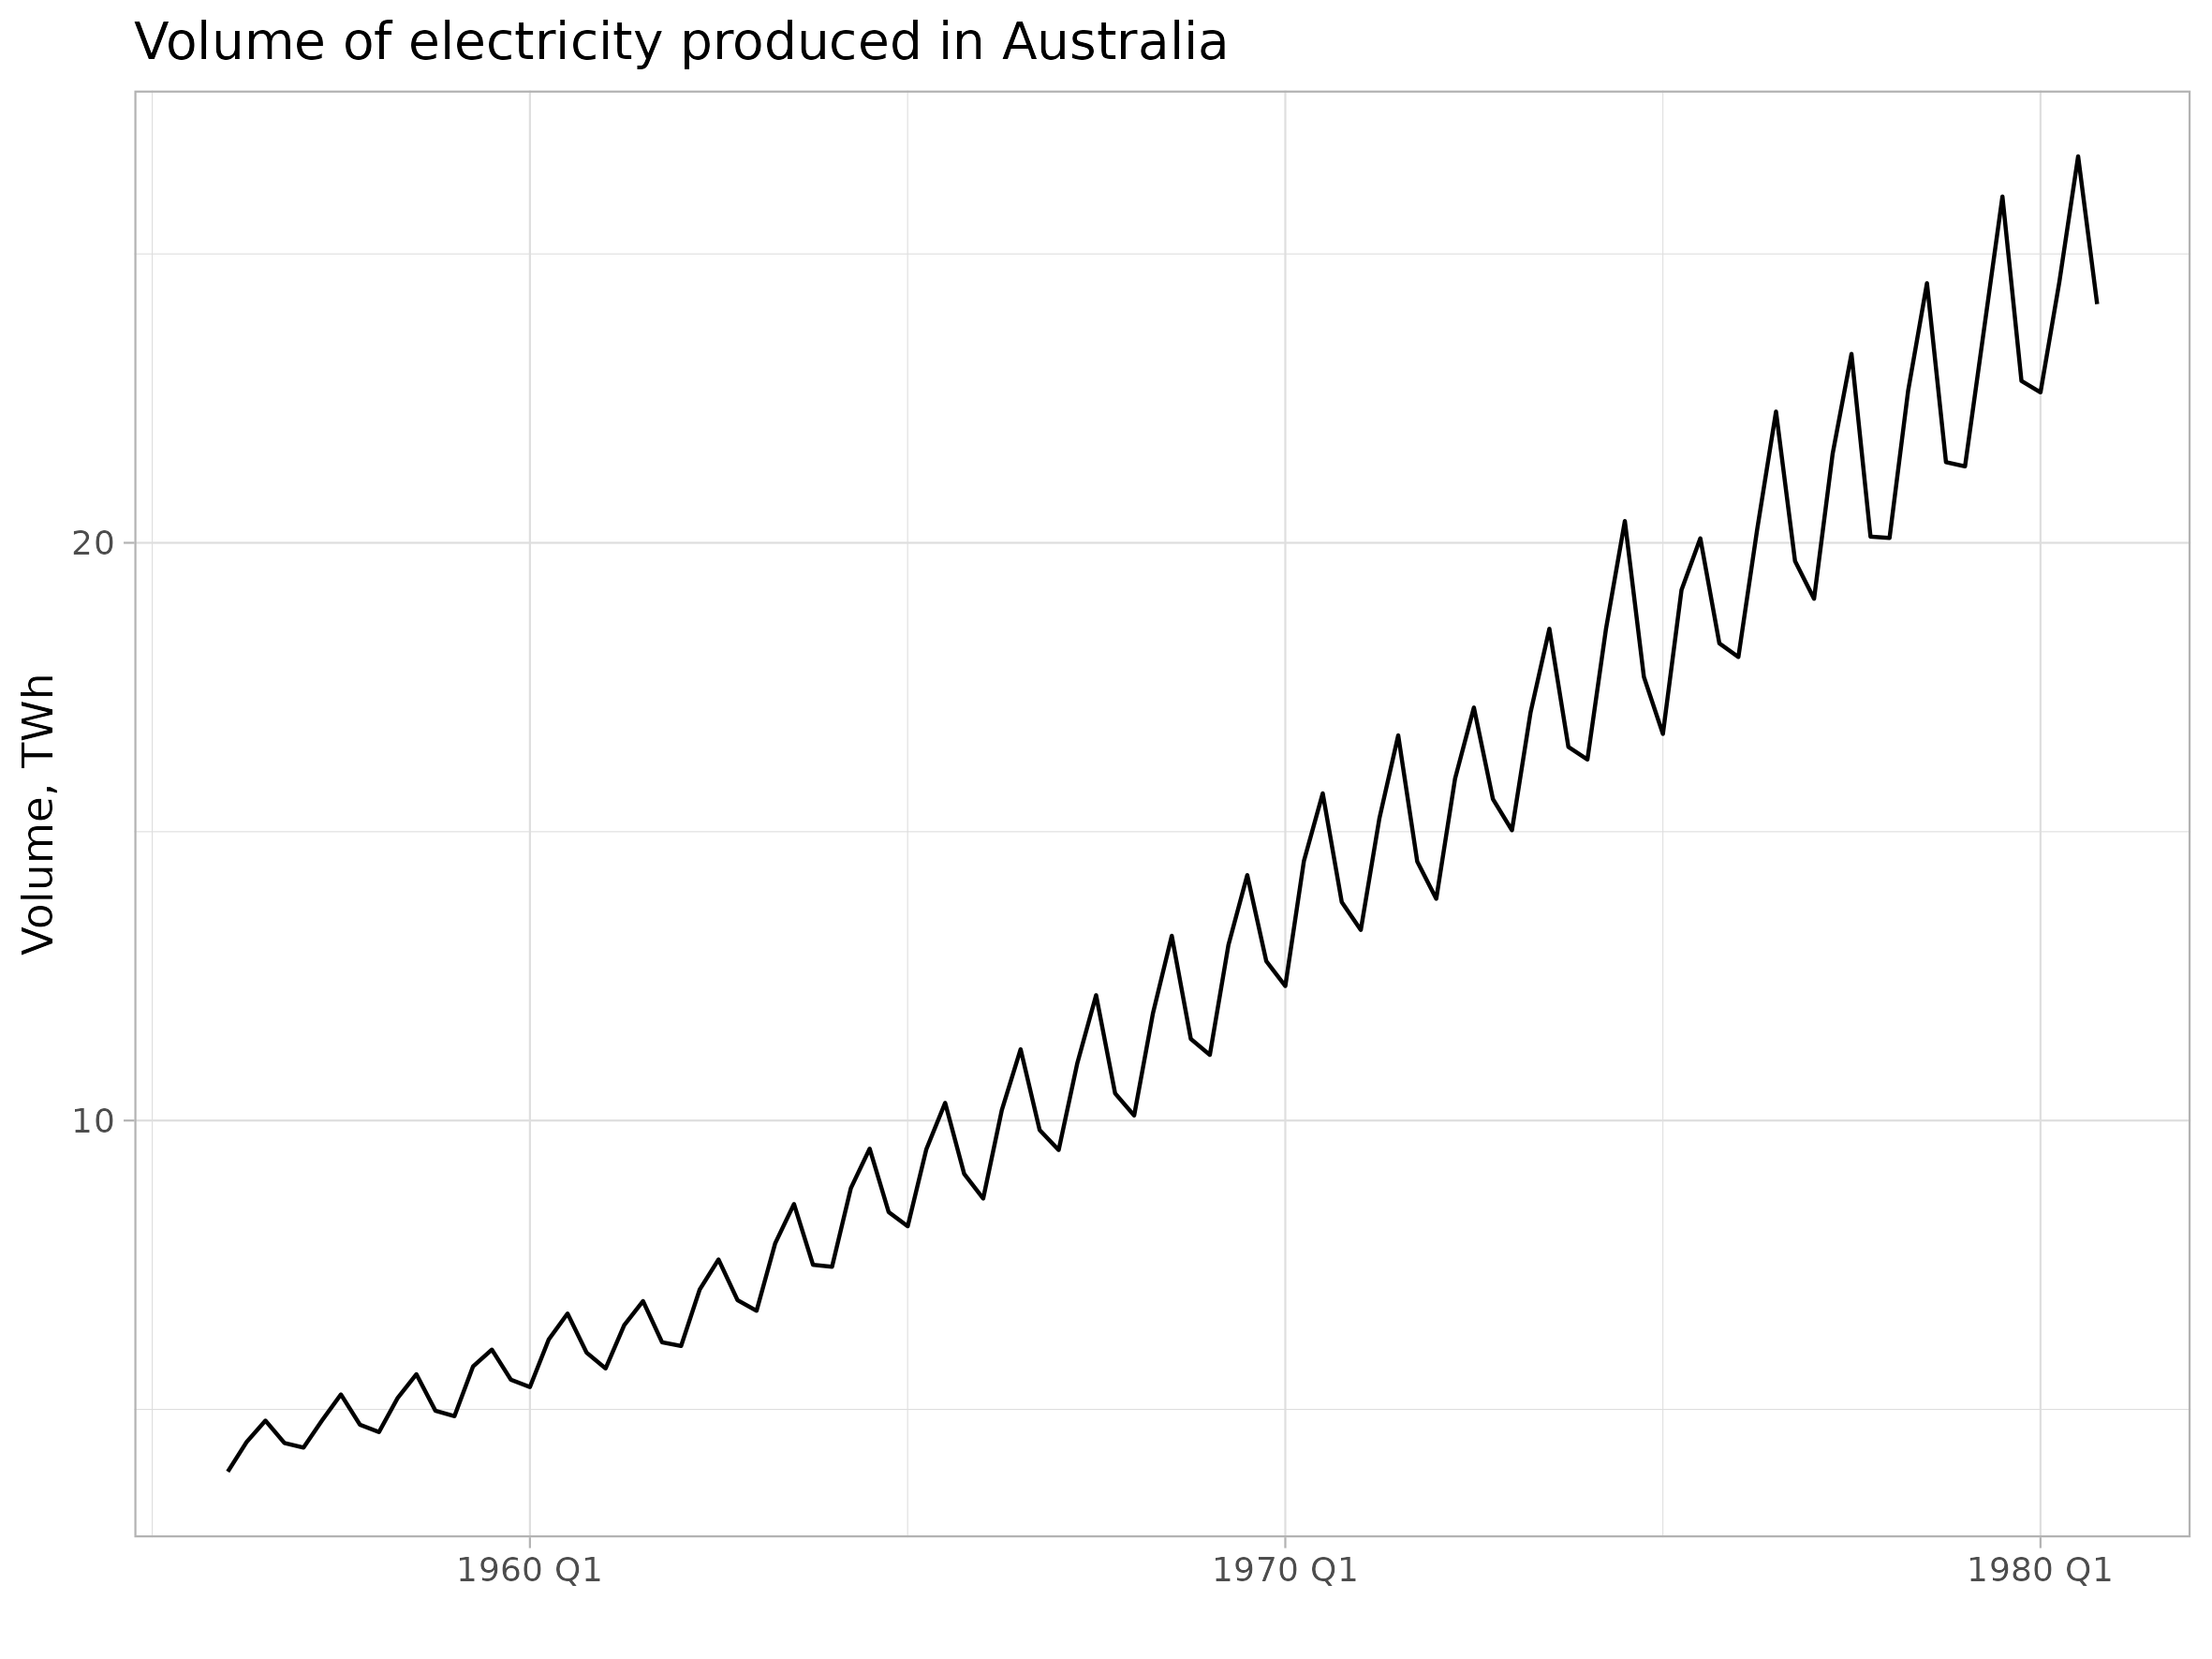
\includegraphics[width=\textwidth]{pictures/om_ts_03-033.png}
	
\end{frame}


\begin{frame}
	\frametitle{Various oscillation amplitude}
	
	Possible \alert{solutions}:
	\begin{itemize}[<+->]
		\item Switch to logarithms, $y_t \to \ln y_t$
		\item Box-Cox transformation, $y_t \to bc(y_t, \lambda)$
		\item Multiplicative components
	\end{itemize}
	
\end{frame}



\begin{frame}
	\frametitle{ETS(MNM): equations}
	
	ETS(MNM) for monthly data:
	
	\[
	\begin{cases}
		y_t = \ell_{t-1} \cdot s_{t-12} \cdot (1 + u_t); \\
		\ell_t = \ell_{t-1}\cdot (1 + \alpha u_t), \text{ starts at } \ell_0; \\
		s_t = s_{t-12}\cdot (1 + \gamma u_t), \text{ starts at } s_0, \ldots, s_{-11}; \\
		u_t \sim \dN(0;\sigma^2) \text{ and are independent} \\
	\end{cases}
	\]
	
	\pause
	ETS(ANA):
	\[
	\begin{cases}
		y_t = \ell_{t-1} + s_{t-12} + u_t; \\
		\ell_t = \ell_{t-1} + \alpha u_t, \text{ starts at } \ell_0; \\
		s_t = s_{t-12} + \gamma u_t, \text{ starts at } s_0, \ldots, s_{-11}; \\
	\end{cases}
	\]
	
\end{frame}





\begin{frame}
	\frametitle{Units}
	
	Series $y_t$, $\ell_t$ — \alert{initial} units.
	
	\pause
		
	The $s_t$ series is measured relative to one, for example, $s_t = 0.9$ — 10\% below the trend.
	
	The $u_t$ series is measured relative to zero, for example, $u_t = -0.1$ — a 10\% drop.
	
\end{frame}



\begin{frame}
	\frametitle{ETS(MNM): Forecasting}
	
	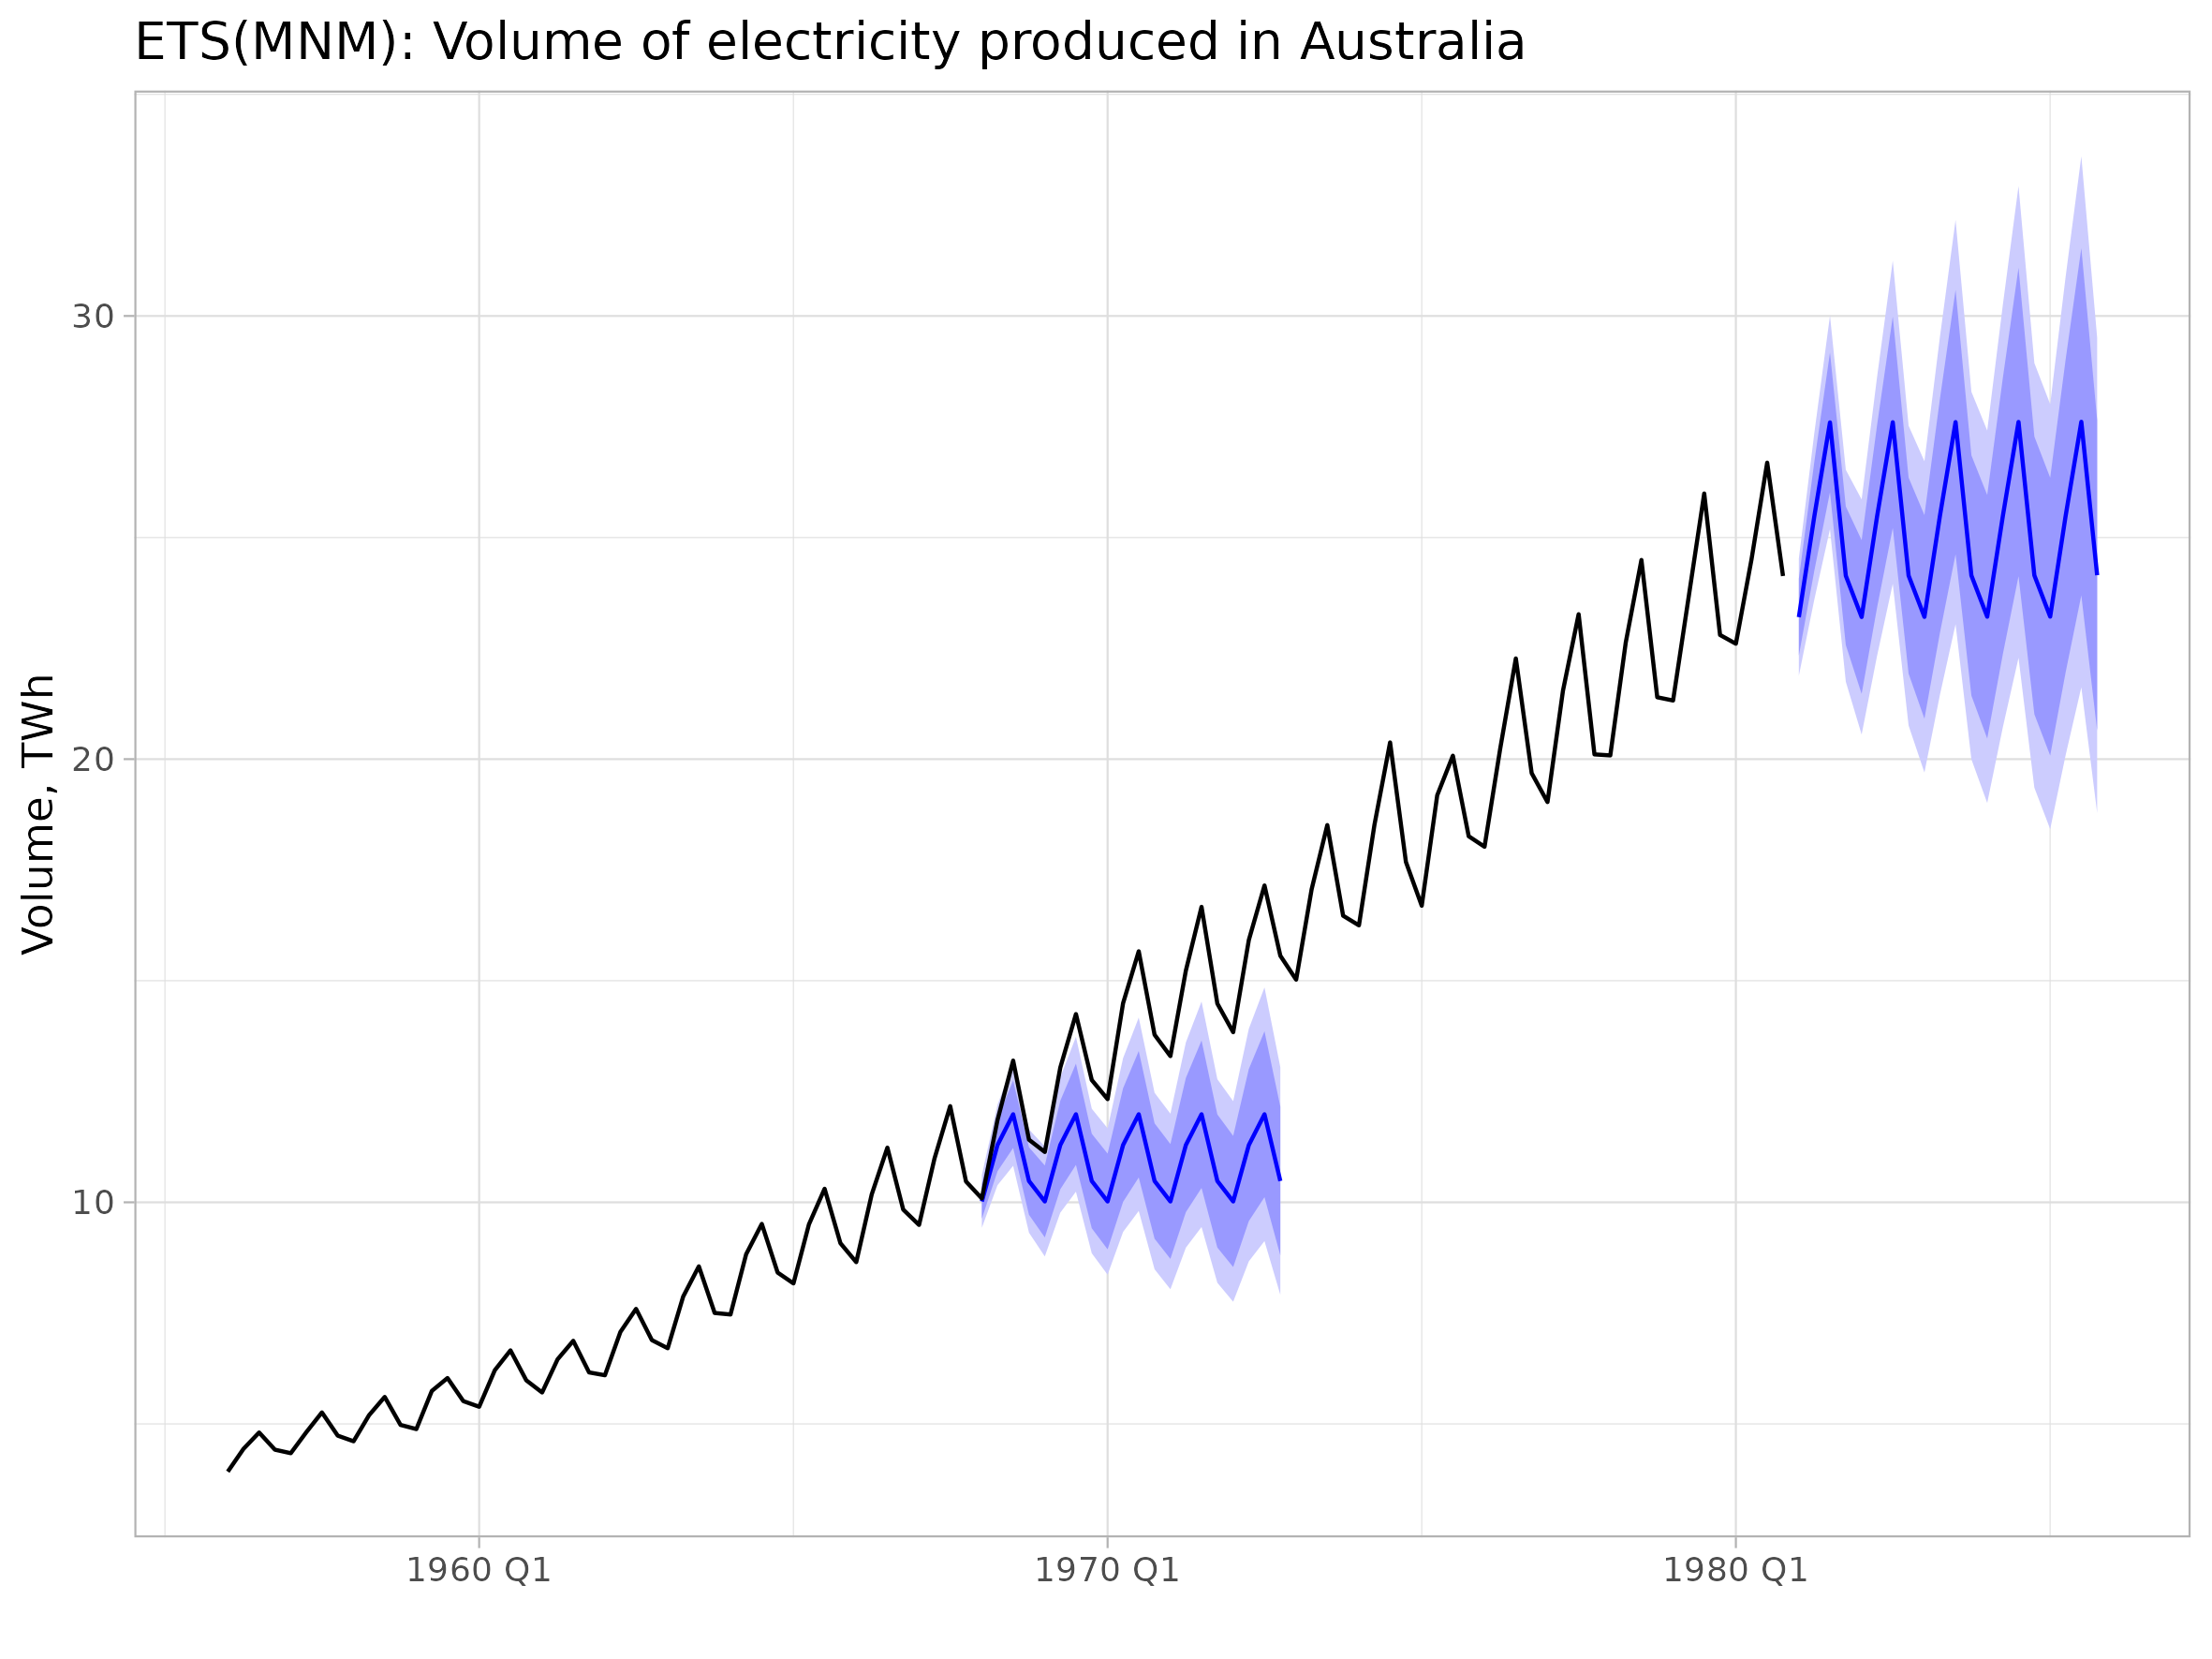
\includegraphics[width=\textwidth]{pictures/om_ts_03-047.png}
	
	
\end{frame}


\begin{frame}{Which option to choose?}
	
	\alert{Different amplitude} of fluctuations: indication of multiplicative models.
	
	\pause
	
	Automatic selection based on the \alert{AIC} criterion works.
	
	\pause
	
	
	You can get the ETS(AAdA) model \alert{with seasonality}.
	
	\pause
	
	Some of the multiplicative models can be \alert{numerically unstable}
	or \alert{not implemented} in the software.
	
\end{frame}



\begin{frame}{ETS Model: Summary}
	
	\begin{itemize}[<+->]
		\item The slope of the trend  and seasonality may change
		\item Automatic decomposition into components
		\item Multiplicative models take into account \alert{changing} oscillation amplitudes
		\item A lot of possible \alert{combinations}
	\end{itemize}
\end{frame}




